\documentclass[conference,10pt]{IEEEtran}
\IEEEoverridecommandlockouts
\usepackage[T1]{fontenc}
\usepackage{graphicx,booktabs,amsmath,amssymb,multirow,xcolor,url,xspace}
\usepackage[hidelinks]{hyperref}
\hypersetup{pdftitle={Egocentric Human Demonstrations for a Bimanual Robot, Part II: Single-Arm Approach}, pdfauthor={Jeong Hwan Lee}}
\usepackage{tikz}
\usetikzlibrary{positioning,arrows.meta,fit,backgrounds}
\newcommand{\mm}{\,mm\xspace}

\begin{document}
\title{Egocentric Human Demonstrations for a Bimanual Robot\\Part II: Single-Arm Approach to a Cube}
\author{\IEEEauthorblockN{Jeong Hwan Lee}
\IEEEauthorblockA{Technical report, version 4, 7 October 2026 \quad alnrg2arg@gmail.com\\
Part I covers three-cube stacking. Code, results and sample data are available on request.}}
\maketitle

\begin{abstract}
Part I showed that, once egocentric human data and robot data share one action contract, the remaining gap is visual and
geometric rather than kinematic. Part II isolates the simplest transferable behaviour: the right arm approaching a red cube,
learned from egocentric human demonstrations only. We report three iterations. (1) HRA\_red: 200 right-hand takes in which
IMU visual--inertial scale turned out to be unobservable (median 0.012, non-positive in 95 takes); scale from a 3.8\,cm cube
of known size replaces it (PnP/IMU ratio 1.06 on bimanual takes where the IMU is reliable) and 166 takes survive. A 0.9B X-VLA
model trained on them overfits from the first checkpoints (held-out loss 0.150 at 15k rising to 0.299 at 105k). On the robot
it moved towards the cube from a nearby start but dragged along the table for far cubes, and calibrating the robot
(head camera, wrist hand-eye with 0.16\,px RMS) exposed several convention errors, including an 82\mm offset between the
forward-kinematics TCP and the physical jaw tip. (2) Wrist images re-rendered with the measured robot camera model and
labels expressed as robot-TCP poses through the hand-eye transform. (3) HRA\_A100: a new protocol in which every take starts
with the gripper tip held on a taped origin that the robot has also touched, giving a shared task frame (collinearity
0.38\mm), per-episode origin yaw (error p50 0.21\textdegree) and a second scale source from the table plane (ratio to cube
PnP 0.999). A table-aware conversion keeps 86 of 107 takes with a fingertip clearance of at least 7.6\mm. Start- and
origin-anchored state give the same held-out loss (0.124 versus 0.132 at 5k), and both overfit from 5k. Robot runs used a
cube-size stop as a proximity proxy (69 of 127 sessions on the last day ended on it), but no trial outcome was logged, so we
report no success rate. Most of what we learned is about frames, scale and deployment settings, which we list with the
corrections we had to make.
\end{abstract}

\section{Introduction}\label{sec:intro}
A reaching motion towards a visible object is the first segment of almost every manipulation task and the simplest one in which human-to-robot transfer~\cite{kareer2024egomimic} can be judged by eye: the arm either moves towards the cube or it does not. Part I found that an
ego-only stacking model gives no useful action direction on robot camera frames (median cosine $-0.05$/$-0.03$), and that the
gap follows the wrist images. A single-arm approach task lets us attack that gap with far fewer confounds: one arm, one object,
no grasp, no task order. The question of Part II is: \emph{can a right-arm approach prior, learned only from egocentric human
demonstrations, move the robot towards the cube, and what has to be true of the data for that to work?}

Our contributions are: a metric-scale source for slow motions that does not depend on the IMU (Sec.~\ref{sec:scale}); a
calibration chain that puts human and robot data in one task frame (Secs.~\ref{sec:robotcal} and \ref{sec:a100}); three
dataset generations with their training behaviour (Secs.~\ref{sec:v1}--\ref{sec:a100}); and the deployment settings and
corrections that turned out to matter (Secs.~\ref{sec:deploy}--\ref{sec:corr}). We report no success rate: the trial logger
of the deployment interface was not used during these runs.

\section{Setup}\label{sec:setup}
\textbf{Device and poses.} The operator wears one HandUMI unit, a UMI-style~\cite{chi2024umi} hand-worn gripper (Part I, Sec.~III), on the right hand: a 1080p30 fisheye wrist
camera, a 200\,Hz IMU and a jaw encoder; a fixed Logitech C922 records the table. Wrist poses come from MASt3R-SLAM~\cite{murai2025mast3rslam} on the RGB
video alone; Part I describes the pipeline.

\textbf{Action contract.} We keep Part I's 20-dimensional Cartesian contract (CART20): rows at 15\,Hz, a chunk of 16 relative
poses $T(t)^{-1}T(t+k\Delta)$ with $\Delta=50.05$\,ms, position, 6-D rotation and gripper per arm. For a right-only task the
left arm is a dummy (identity pose, gripper 0) and is masked out of the loss together with the gripper (jaw unused), so 9 of the
20 dimensions are supervised. The task string is ``Approach to the red cube''.

\textbf{Model and training.} X-VLA~\cite{zheng2025xvla} (0.9B, LeRobot) with Part I's recipe: soft-prompt slot 20, batch 8, 8-bit AdamW (policy
learning rate $10^{-4}$), bf16, seed 1000, a checkpoint every 5k steps, on an RTX~4090. A 300-step smoke test verified the loss
mask: masked and padded dimensions receive exactly zero gradient and every supervised dimension a non-zero one.

\textbf{Robot.} The reBot B601 right arm with a wrist C922, driven from a Mac through a pink IK solver. On the robot the left arm
is locked and both jaws hold; the deployment interface refuses any command for them.

\section{HRA\_red: Object-Based Scale}\label{sec:scale}
We recorded 200 right-hand takes of ``approach the red cube'' (10\,s each) in one session on 3 October.

\textbf{IMU scale fails on slow motion.} The per-episode visual--inertial scale that works on the stacking data is
unobservable here: the approaches are slow and smooth, so the accelerometer barely constrains it. Across the 200 takes the IMU
scale has a median of 0.012 and is zero or negative, which is physically impossible, in 95 of them (Fig.~\ref{fig:cube}b).

\textbf{Scale from a known cube.} The red cube is static and has a 3.8\,cm edge. In frames where it is visible we fit its
silhouette with a two- or three-face model, or a single-face model when one face is seen within 35\textdegree{} of head-on,
solve PnP, and recover the trajectory scale in closed form from the requirement that the cube stays put. An episode is valid
with at least 10 PnP frames, a bootstrap spread of at most 10\% and a cube-centre residual of at most 2\,cm. On the bimanual
HRL80 stacking takes, where the IMU scale is reliable, 37 of 57 right-hand episodes are PnP-valid and the PnP/IMU ratio has a
median of 1.062 (p16--p84 0.959--1.274; Fig.~\ref{fig:cube}a).

\begin{figure*}[t]
\centering
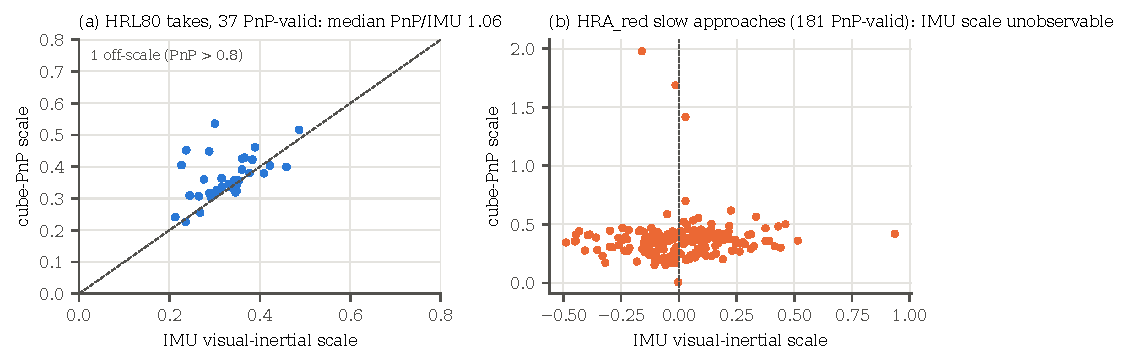
\includegraphics[width=\textwidth]{figures/fig6_cube_scale.pdf}
\caption{Per-episode metric scale of the MASt3R-SLAM trajectory from the IMU and from cube PnP. (a) HRL80 stacking takes,
where the IMU scale is reliable. (b) HRA\_red approach takes: the IMU scale scatters around zero.}
\label{fig:cube}
\end{figure*}

\textbf{Funnel.} Of 200 takes, 19 fail the scale gates (14 with too few PnP frames, 5 with too large a spread) and 15 fail a
physical sanity check on the scaled trajectory (scale between 0.1 and 1.0, SLAM travel at least 0.8 of the PnP-observed
approach distance, travel at most 0.8\,m). The remaining 166 are split into 151 train episodes (20{,}319 rows) and 15
validation episodes (2{,}011 rows). The median scale is 0.354 (p5 0.188, p95 0.500) and the median cube-centre residual 0.17\,cm.

\section{HRA\_red v1: Training and First Robot Runs}\label{sec:v1}
\textbf{Training.} In v1 the wrist fisheye frames were re-rendered as a pinhole view with a \emph{guessed} robot camera
(62--70\textdegree{} horizontal field of view, principal point shifted so that the jaws sit low in the image), as for
ROBOT100 in Part I. The 300k-step run finished on 5 October at a training loss of 0.002 (118 epochs). Held-out loss rises from
the first evaluated checkpoint (Table~\ref{tab:val}, Fig.~\ref{fig:val}a): 0.150 at 15k (training subset 0.066), 0.198 at 30k,
0.213 at 60k, 0.265 at 90k and 0.299 at 105k, while the training-subset loss falls to 0.018. With 151 episodes the model
overfits almost immediately; checkpoints below 15k were not evaluated.

\begin{table}[t]
\centering\footnotesize\setlength{\tabcolsep}{3pt}
\caption{Held-out loss (masked MSE on the 9 supervised dimensions) by checkpoint; training-subset loss in parentheses.}
\label{tab:val}
\resizebox{\columnwidth}{!}{\begin{tabular}{@{}lccccc@{}}
\toprule
Dataset (val eps) & 5k & 15k & 30k & 45k/50k & 105k \\
\midrule
HRA\_red v1 (15) & -- & 0.150 (0.066) & 0.198 (0.053) & -- & 0.299 (0.018) \\
A100 A: start (11) & 0.124 (0.110) & 0.125 (0.058) & 0.141 (0.031) & 0.224 (0.020) & -- \\
A100 B: origin (11) & 0.132 (0.097) & 0.147 (0.057) & 0.174 (0.031) & 0.190 (0.022) & -- \\
\bottomrule
\end{tabular}}
\end{table}

\textbf{First robot runs.} Checkpoints from 15k to 75k ran 8{,}397 control cycles (658 run starts) on 4 October, and v1 100k,
200k and 300k ran 61 planned sessions on the afternoon of 6 October while we tuned the chunk-execution settings
(Sec.~\ref{sec:deploy}); the operator's verdicts were ``accuracy dropped a lot'' and ``too much zigzag''. From a start near
the cube the arm moved towards it; for cubes far to the left it dragged along the table, by about 39 and 26\,cm in two runs.
None of these runs has a logged outcome.

\section{Calibrating the Robot Side}\label{sec:robotcal}
Interpreting those runs required knowing where the human data sits relative to the robot, which v1 never did: its labels are
relative motions of the UMI tool frame, and its start state is the human's own start.

\textbf{Head camera.} The fixed C922 (the same camera and position as during HRA\_red) was calibrated with an 8$\times$5
checkerboard of 25\mm squares (48 frames, RMS 1.05\,px, $f=728.7$\,px), and its pose in the robot base was found by touching
four board corners with the TCP (residuals 2--6\mm).

\textbf{Linking human takes to the base.} For each take we detect the cube in the head camera, place it in the robot base, and
attach the wrist trajectory through the wrist-camera cube PnP; tilt comes from IMU gravity against the table normal, yaw from
the cube faces. This linked 64 of 166 takes (head-camera detection is the bottleneck) and exposed an 18\textdegree{} rotation
error in the exported camera--IMU extrinsic (cube-axis error 17.8$\to$3.4\textdegree{} after correction); earlier IMU-based
tilt statistics are wrong by up to that amount. Training poses were unaffected because their scale comes from cube PnP. The
link was later judged too noisy to build a dataset on (start heights spread over 4\,cm, up-axis error p50 10\textdegree,
p90 28\textdegree), which motivated the protocol of Sec.~\ref{sec:a100}.

\textbf{Robot wrist hand-eye.} Thirteen board views give a wrist-camera calibration with 0.16\,px RMS ($f=651.4$\,px) and a
hand-eye transform on which four methods (including Tsai--Lenz~\cite{tsai1989handeye}) agree (board-in-base spread 1--2\mm, 0.3\textdegree). The camera sits 169.5\mm
behind the TCP and 76\mm off its axis, and its optical axis points 33\textdegree{} below the TCP $x$ axis. The human wrist
camera at the take start and the robot wrist camera at a reachable start cannot be made to coincide: matching the human's
view would need the shoulder joint past its limit. The closest feasible start (pose A) puts the camera within 1--14\mm in the
horizontal plane but 78\mm higher and 8\textdegree{} steeper.

\textbf{TCP is not the jaw tip.} The IK stack's TCP lies about 82\mm ahead of the physical jaw tip along the TCP $x$ axis
(found by projecting FK points into the wrist image). Several readings of ``the tip goes below the table'' were this artefact
and were retracted. The contact model now uses the URDF fingertip box (70--80\mm behind the TCP, $\pm$19.6\mm), whose lowest
corner counts as contact.

\textbf{Re-reading the v1 runs.} With pose A and the jaw-tip model, one run each of v1 200k with three conventions gave: tool
axis unrotated, the tip ended about 2\,cm from the cube and 3\,cm above the table; rotated by the 33.1\textdegree{} camera
pitch, it overshot by about 11\,cm; rotated and offset by the camera--TCP translation, it ended about 4\,cm from the cube and
10\,cm above the table. These are single runs reconstructed from forward kinematics, not measurements of success.

\section{Robot-Camera Rendering (robotcam v2)}\label{sec:v2}
v1 rendered the wrist view with a guessed camera. The measured robot C922 has a 52\textdegree{} horizontal field of view with
a centred principal point, so v1 showed the cube much later in the approach than the robot camera does. In v2 every wrist
frame is rendered with the measured intrinsics and the hand-eye pose, and labels are expressed as robot-TCP poses through the
hand-eye transform (robot TCP $\to$ UMI TCP: $-33$\textdegree{} about $y$, $t=(-94.8, 2.4, 38.4)$\mm). The 151/15 split is
unchanged. A run on v2 reached about 64k steps (training loss 0.026) before being stopped; a version mixing v2 with the first
A100 takes was rejected because the two collections have no common origin (next section).

\section{HRA\_A100: A Shared Origin}\label{sec:a100}
\textbf{Protocol.} A cross of tape on the head-camera base plate, about 35\,cm from the robot gripper, is the task origin.
Each take is an automatic cycle: 5\,s rest; the operator places the HandUMI jaw tip on the cross and holds it still for
2\,s; recording starts with a further 2\,s hold inside the recording (the origin); a 3\,s ``ready'' phase moves the hand to a
robot-like start pose; at ``go'' a 10\,s approach is recorded, and training data starts at ``go''. Cube placements were planned
as 40 centre, 20 left/right, 20 front/back and 20 edge. On 6 October 107 takes were kept in four sessions (7, 8, 9 and 83
takes; the first session predates the origin hold).

\begin{figure}[t]
\centering
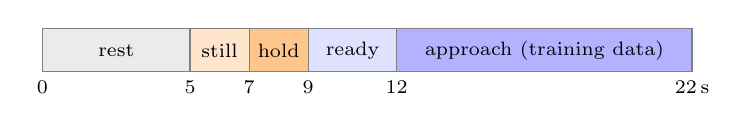
\begin{tikzpicture}[font=\scriptsize, x=0.375cm]
\foreach \a/\b/\t/\c in {0/5/rest/black!8, 5/7/still/orange!20, 7/9/hold/orange!45, 9/12/ready/blue!12, 12/22/approach (training data)/blue!30}
  {\fill[\c] (\a,0) rectangle (\b,0.55); \draw[black!50] (\a,0) rectangle (\b,0.55); \node at ({(\a+\b)/2},0.27) {\t};}
\foreach \x/\l in {0/0, 5/5, 7/7, 9/9, 12/12, 22/22\,s} \node[below] at (\x,0) {\l};
\end{tikzpicture}
\caption{HRA\_A100 take cycle: rest, jaw tip still on the taped cross, recording starts with a 2\,s origin hold, ready, 10\,s approach. The origin hold places the HandUMI jaw tip on the same taped cross that the robot jaw tip touched
during calibration.}
\label{fig:protocol}
\end{figure}

\textbf{Task frame G.} The robot's right jaw tip touched three points on the tape line (far, centre, near); they are collinear
to within 0.38\mm over a 60.4\mm baseline and agree in height within 2\mm. G has its origin at the cross centre, $x$ along the
tape towards the human side and $z$ along base $z$: origin $(59.0, -74.9, 6.2)$\mm in the robot base, heading
47.09\textdegree. With the 35\mm plate the table is at $z=-27.1$\mm.

\textbf{Scale and orientation at the origin.} During the hold the fingertip is on the plate, so the first MASt3R keyframe's
pointmap contains the table plane at a known distance from the camera. Fitting up to three planes by RANSAC (excluding the
finger) and taking the largest one parallel to the plate gives a second scale source; against cube PnP on 40 takes its ratio
has a median of 0.999 and a per-episode error of p50 8\%, p90 37\%. Each episode uses cube PnP where it is valid and the
origin plane otherwise (35 and 72 of 107); the IMU is not used. The origin yaw is measured per episode by matching the table
around the cross (error p50 0.21\textdegree, p90 1.17\textdegree); assuming a mean yaw instead had produced false rejections
and a 57\mm endpoint-height spread (35\mm with measured yaw). The hold itself repeats to 14\mm (p50; p90 37\mm) and
6.2\textdegree{} (p50), with the camera pitched 63.7\textdegree{} down.

\textbf{Start-anchored versus origin-anchored state.} On 93 takes (82 train, 11 validation; the excluded 14 are the old
session, 7 takes in which the hand moved over 20\mm during the hold, and one physics failure) we trained two otherwise identical
models: A anchors the state at the hand pose at ``go'', B at a fixed origin frame F (the cross, with the tape heading and the
median hold pitch). Both use robot-TCP labels and the robot-camera rendering. Their held-out losses are close and both are
lowest at the first checkpoint (Table~\ref{tab:val}, Fig.~\ref{fig:val}b): A 0.124 and B 0.132 at 5k, rising to 0.224 (A, 50k)
and 0.190 (B, 45k). With 82 training takes, both models overfit from 5k steps. Neither anchoring is better on this measure.

\begin{figure*}[t]
\centering
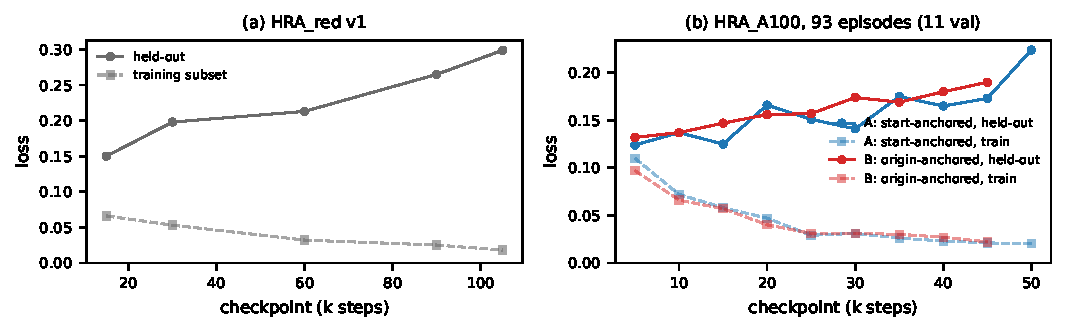
\includegraphics[width=0.8\textwidth]{figures/fig9_hra_val.pdf}
\caption{Held-out (solid) and training-subset (dashed) loss by checkpoint. (a) HRA\_red v1, 15 validation takes. (b) HRA\_A100,
start-anchored (A) and origin-anchored (B) state, 11 validation takes. All runs overfit from the earliest checkpoint.}
\label{fig:val}
\end{figure*}

\textbf{Table-aware conversion.} Expressing human motion in G and starting it from a robot start pose can push the fingertip
into the table. The conversion therefore re-anchors the start to the robot start pose with a weight that decays to zero over the
take, so the human endpoint near the cube is kept, and solves a small quadratic program per take with a hard floor at the
table plus 5\mm and a preferred clearance of 12\mm; an endpoint may be lifted by at most 30\mm. Table~\ref{tab:ct} shows the
variants. CT4 decays position, height and rotation on separate schedules; CT5 adds measured origin yaw, the corrected IMU
gravity, absolute state in G and an origin-hold gate (hold within 10\mm of the origin); CT6 moves the robot start 6\,cm back and
4\,cm down. CT5 and CT6 keep 86 takes with fingertip clearance p50 12.6\mm and minimum 7.6\mm; most rejections are the old
session or takes whose origin yaw could not be measured.

\begin{table}[t]
\centering\footnotesize\setlength{\tabcolsep}{3pt}
\caption{Table-aware conversions of HRA\_A100. Accepted = PASS + PASS-CORRECTED. Clearance: fingertip above the table after
correction, accepted takes.}
\label{tab:ct}
\resizebox{\columnwidth}{!}{\begin{tabular}{@{}lcccc@{}}
\toprule
Variant & Takes & Accepted & Main rejections & Clearance p50 / min \\
\midrule
C (mean yaw) & 107 & 81 & lift $>$30\,mm 10, old 7 & 19.5 / 7.0\mm \\
CT4 (per-axis decay) & 107 & 87 & lift 10, old 7 & 20.6 / 7.9\mm \\
CT5 (yaw, G, hold gate) & 107 & 86 & yaw not measured 9, old 7 & 12.6 / 7.6\mm \\
CT6 (start back/down) & 107 & 86 & as CT5 & 12.6 / 7.6\mm \\
CT7 (low start, +27) & 134 & 90 & IK 19, yaw 11, old 7 & 12.4 / 7.6\mm \\
\bottomrule
\end{tabular}}
\end{table}

\textbf{Start pose.} Where the robot starts matters for both views and reachability. We compared ten candidate start poses
derived from the median and medoid of the human ``go'' poses in G, moved back, right and down. The operator preferred the
lowest (pose 08, TCP $(273, -168, 116)$\mm, joint margin 9.1\textdegree). On 7 October 27 further takes were recorded with a
lower human start (origin to ``go'' about 89\mm instead of about 247\mm); from pose 08 only 5 of them pass, so they were dropped,
and the current run (CT7-old, 85 takes from 6 October, start 08, 100k-step schedule) uses only the 6 October data. CT5 and CT6
runs were stopped after 7k and 3k steps while settings changed; there is no validation split for CT6 and CT7.

\section{Deployment Settings That Mattered}\label{sec:deploy}
\textbf{Chunk execution.} The interface blends successive 16-step chunks. With an exponential blend of 0.25, no cross-fade, no
smoothing and a minimum of one executed row per chunk, motion was acceptable; with the code defaults (0.35, 4 rows, 3\textdegree,
6 rows), which a restart of the interface silently restored on 7 October, the operator reported that ``inference quality had
dropped a lot'' until the values were restored. Inference quality on the robot therefore depends on settings that are not
part of the checkpoint; the loader now restores them.

\textbf{Tool-frame convention.} Models trained on robot-TCP labels (v2, A100) must run with zero camera pitch and zero
camera--TCP offset; the 33.1\textdegree{} pitch and offset of Sec.~\ref{sec:robotcal} apply only to v1. Anchored models must be
served with the same anchor file (F for B, G for CT5--CT7).

\textbf{Cube-size stop.} On 7 October the operator observed the arm pushing the cube instead of stopping. Every 0.1\,s the
interface now measures the red cube's apparent size ($\sqrt{\text{area}}$ in pixels on the raw 640$\times$480 wrist frame) and
stops when two readings exceed a threshold (170--250\,px were used); in follow mode it resumes when the cube shrinks below 85\%
of the threshold. A cube-size stop means the cube looks large in the wrist view; it is a proximity proxy, not verified contact.
The wrist image was also zoomed 1.5$\times$ because the cube looked smaller than in training at the same position.

\textbf{Guards.} During v1 the interface stopped a run after 450\mm net travel, 80\mm between inferences, a still period, or
an output above 250\mm or 60\textdegree; a 6\,s time limit ended runs after 1--4 cycles and was removed. For A100 models all
numeric guards are off and the left arm and jaws stay locked.

\section{Robot Observations}\label{sec:robot}
The interface's planned-execution log records 192 sessions on 6 and 7 October. On 6 October, 65 sessions (v1 checkpoints, the
chunk-setting tuning above) were all stopped by the operator except one, which the interface closed when a planned row jumped by
90.9\textdegree. On 7 October, 127 sessions ran: B 45k (3), A 50k (6) and CT5 5k (4), then B 50k with the 1.5$\times$ zoom (114
sessions, many of them follow-mode resumes); 69 of the 127 ended on the cube-size stop and 58 were stopped by the operator.
The log has no outcome field and the trial logger was not used, so we cannot say how many approaches reached the cube, and we
report no success rate. The cube appears orange in the fisheye-rendered training images and red on the robot camera, a colour
gap we have not corrected.

\section{Corrections}\label{sec:corr}
Several of our own intermediate readings were wrong, each found by an independent check: the robot start tilt was 25\textdegree,
not 3\textdegree; the robot's wrist view is about 1.32$\times$ magnified and 11\textdegree{} lower than the human's, not
2.5$\times$; ``labels drive the tip 5\,cm into the table'' was the TCP--tip offset; the table height moved from $-54.3$ to
$-5.9$ to $-27.1$\mm as the contact model was fixed; IMU tilt statistics were off by up to 18\textdegree; and a mean origin yaw
caused false rejections. We list them because the same errors are easy to make in any human-to-robot calibration.

\section{Lessons}\label{sec:lessons}
(i) \emph{Every scale source has a regime in which it fails silently}: the IMU on slow motion, cube PnP on oblique single-face
views, the origin plane on a few takes (p90 error 37\%); a second independent source is needed to see the failure.
(ii) \emph{A shared physical origin is cheaper than post-hoc registration}: linking 166 takes after the fact through a head
camera reached 64 takes with centimetre errors, while a taped cross touched by both the robot and the human gives a common
frame with sub-millimetre line fit. (iii) \emph{The TCP of the IK stack is a convention, not the fingertip}; contact
reasoning needs the fingertip geometry. (iv) \emph{Small single-task sets overfit at once}: with 80--150 takes, held-out loss
is lowest at the first checkpoint (5k or 15k), so the early checkpoints are the ones to test on the robot. (v) \emph{Execution
settings are part of the policy}: blend and smoothing parameters that live in the interface changed robot behaviour more than
a change of checkpoint, and must be recorded with every run.

\section{Limitations and Next Steps}\label{sec:lim}
We have no success rate and no controlled comparison of datasets on the robot: runs were exploratory, settings changed between
them, and outcomes were not logged. The A100 data come from one operator, one scene and two days; the held-out sets are 11--15
takes. The cube colour differs between the rendered training images and the robot camera. The approach data teach a direction
towards one red cube; they make no claim about colour grounding. Next: log every robot trial (checkpoint, start pose, cube
position, reached yes/no, stop reason) with fixed execution settings; test early checkpoints (5k--15k) of A, B and CT7 from
the same start poses and cube positions; collect more A100 takes from the chosen start; correct the colour of the rendered
wrist images; and then use the approach prior as the first segment of the stacking policy of Part I.

\section{Conclusion}
For a single-arm approach, egocentric human data can be brought into the robot's frame with sub-centimetre consistency, but
only after replacing the IMU scale with object- and plane-based scale, calibrating the robot wrist camera, and anchoring every
take at a physical origin shared with the robot. Models trained on 80--150 such takes overfit quickly, and on the robot they move
towards the cube from nearby starts; with no logged outcomes, how often they reach it is still open.

\begin{thebibliography}{99}\footnotesize
\bibitem{chi2024umi} C.~Chi \emph{et al.}, ``Universal manipulation interface: In-the-wild robot teaching without in-the-wild robots,'' in \emph{RSS}, 2024.
\bibitem{kareer2024egomimic} S.~Kareer \emph{et al.}, ``EgoMimic: Scaling imitation learning via egocentric video,'' \emph{arXiv:2410.24221}, 2024.
\bibitem{zheng2025xvla} J.~Zheng \emph{et al.}, ``X-VLA: Soft-prompted transformer as scalable cross-embodiment vision-language-action model,'' in \emph{ICLR}, 2026 (arXiv:2510.10274).
\bibitem{murai2025mast3rslam} R.~Murai, E.~Dexheimer, and A.~J. Davison, ``MASt3R-SLAM: Real-time dense SLAM with 3D reconstruction priors,'' in \emph{CVPR}, 2025.
\bibitem{tsai1989handeye} R.~Y. Tsai and R.~K. Lenz, ``A new technique for fully autonomous and efficient 3D robotics hand/eye calibration,'' \emph{IEEE Trans. Robotics and Automation}, 1989.
\end{thebibliography}
\end{document}
